
\begin{figure}[H]
\centering
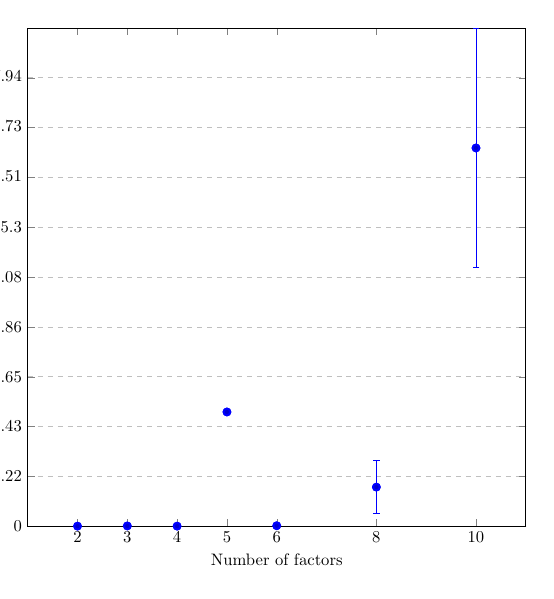
\begin{tikzpicture}[scale=0.6, trim axis left, trim axis right]
\begin{axis}[
    width=1\textwidth,
    height=1\textwidth,
    xlabel={Number of factors},
    ylabel={Time taken (s)},
    xmin=1.0, xmax=11.0,
    ymin=1.3e-05, ymax=1542.158514,
    xticklabels={2, 3, 4, 5, 6, 8, 10},
    xtick={2, 3, 4, 5, 6, 8, 10},
    ytick={1.3e-05, 154.2158631, 308.4317132, 462.6475633, 616.8634134, 771.0792635, 925.2951136, 1079.5109637, 1233.7268138, 1387.9426639},
    ymajorgrids=true,
    grid style=dashed,
]

\addplot+[
    blue,
    very thick,
    forget plot,
    only marks
    ]
    plot[
    very thick,
    error bars/.cd,
    y dir=plus,
    y explicit
    ]
    table[x=x,y=y,y error expr=\thisrow{y-max}] {
    x    y    y-max
    10	1170.7868623	371.3716517
3	0.61735205	0.00865395
2	2.115e-05	8.85e-06
5	353.4699723	3.5083447
4	4.3375e-05	3.3625e-05
6	1.26331195	0.10873605
8	120.8888585	83.3034535

    };

\addplot+[
    blue,
    very thick,
    forget plot,
    only marks
    ]
    plot[
    very thick,
    error bars/.cd,
    y dir=plus,
    y explicit
    ]
    table[x=x,y=y,y error expr=\thisrow{y-min}] {
    x    y    y-min
    10	1170.7868623	-369.3608323
3	0.61735205	-0.00453805
2	2.115e-05	-8.15e-06
5	353.4699723	-4.0354913
4	4.3375e-05	-1.1375e-05
6	1.26331195	-0.04952995
8	120.8888585	-82.4576535

    };

\end{axis}
\end{tikzpicture}
\vspace{-0.3cm}
\caption{Medium primes, close primes}\label{fig:FermatsFactorizationMediumcloseprimesfactors}
\end{figure}
